\section{Fundamentals}

In the section fundamentals, the author explains the necessary theoretical techniques to understand the Generative Adversarial Network framework. The author references essential literature in the GAN research area and introduces the general GAN framework, a often used network architecture, and an improved loss function to train GANs.

\subsection{Generative Adversarial Network}

\citeauthor{goodfellow2014generative} first introduced GANs \cite{goodfellow2014generative}. They created a framework of two Neural Networks which are co-trained. One they call the Generator, it takes a random noise vector as an input and transforms it to generate data in the form of images. The other one they call the Discriminator, which decides if the image is fake or not. It takes data in the form of images and tries to estimate if the given image comes from a real dataset, in their case, the MNIST dataset or from the Generator.\\

In other words the Generator transforms the noise distribution $ p_{z}(z) $ to $ p_{g} $. The learning process then tries to shift $ p_{g} $ towards the real data distribution $ p_{data} $. So that under optimal conditions the $ p_{g} $ and $  p_{data} $ are indistinguishable by the Discriminator.\\

\begin{figure}[H]
    \centering
    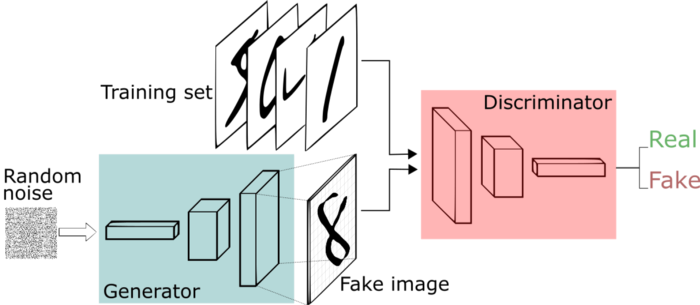
\includegraphics[width=0.65\textwidth]{resources/images/gan.png}
    \caption{Illustration of the general architecture of a Generative Adverserial Network. By \citeauthor{twd:gan} \cite{twd:gan}.}
    \label{fig:gan}
\end{figure}

They use the following training objective in the form of a value function. Their implementation negates the formula to create the corresponding loss function.\\

\begin{equation}
    \min _{G} \max _{D} V(D, G)=\mathbb{E}_{\boldsymbol{x} \sim p_{\text {data }}(\boldsymbol{x})}[\log D(\boldsymbol{x})]+\mathbb{E}_{\boldsymbol{z} \sim p_{\boldsymbol{z}}(\boldsymbol{z})}[\log (1-D(G(\boldsymbol{z})))]
\end{equation}\\

\newpage

To train the GAN, they update the Discriminator more often than the Generator. For each iteration, they alter the Discriminator weights $ k $ times and perform gradient ascend based on the following loss function:\\
unseen images
\begin{equation}
    \nabla_{\theta_{d}} \frac{1}{m} \sum_{i=1}^{m}\left[\log D\left(\boldsymbol{x}^{(i)}\right)+\log \left(1-D\left(G\left(\boldsymbol{z}^{(i)}\right)\right)\right)\right]
\end{equation}\\

Afterward, the Generator is updated once with gradient ascend and the loss function:\\

\begin{equation}
    \nabla_{\theta_{g}} \frac{1}{m} \sum_{i=1}^{m} \log \left(1-D\left(G\left(\boldsymbol{z}^{(i)}\right)\right)\right)
\end{equation}\\

\subsection{Deep Convolutional GAN}

Deep Convolutional GAN (DCGAN) is an advancement of the original GAN model proposed by \citeauthor{goodfellow2014generative}.  \citeauthor{radford2016dcgan} developed it in 2015. Compared to GAN, it uses purely convolutional operations instead of the used Dense-layers in the first GAN architecture.\\

\begin{figure}[H]
    \centering
    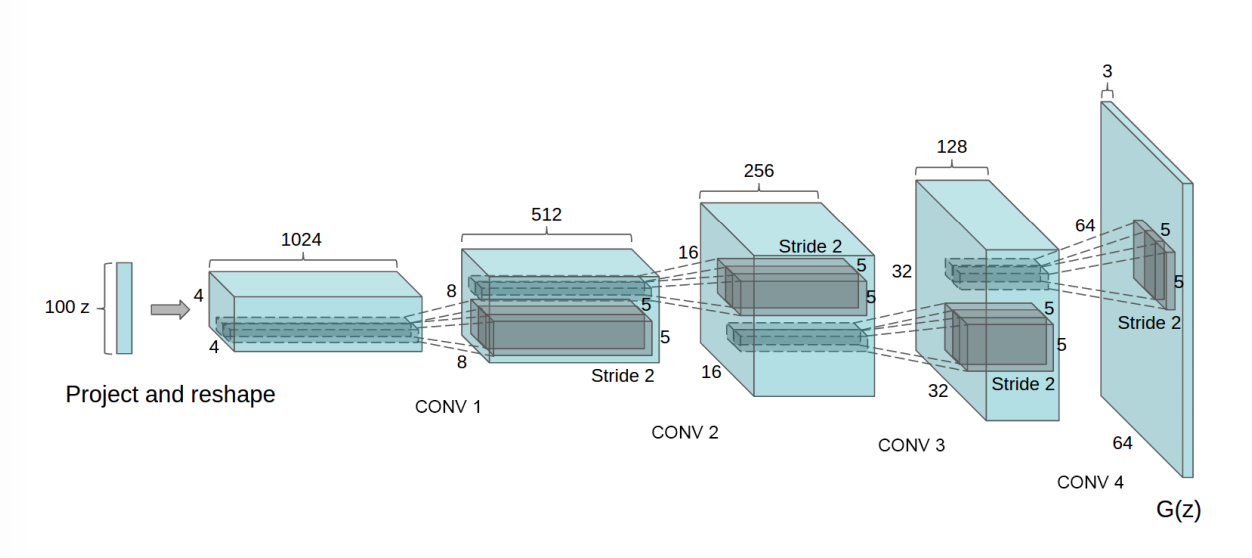
\includegraphics[width=0.65\textwidth]{resources/images/dcgan_generator.png}
    \caption{The Generator architecture proposed by \citeauthor{radford2016dcgan} in \citetitle{radford2016dcgan} \cite{radford2016dcgan}.}
    \label{fig:dcgan_generator}
\end{figure}

\citeauthor{radford2016dcgan} develop the following guidelines for the GAN architecture based on convolutional layers.

\begin{itemize}
    \item Replace any pooling layers with strided convolutions (Discriminator) and fractional-strided convolutions (Generator).
    \item Use batch-normalization in both the Generator and the Discriminator.
    \item Remove fully connected hidden layers for deeper architectures.
    \item Use ReLU activation in Generator for all layers except for the output, which uses Tanh.
    \item Use LeakyReLU activation in the Discriminator for all layers.
\end{itemize}


They claim by applying these guidelines they could improve the stability of the adversarial training. They also identify that sometimes the models collapse to a subset or a single mode if training time was too long.\\

Today's more modern GAN implementations often use DCGAN as a baseline and build their architecture upon the original one. Often the proposed guidelines are partially applied.\\

\subsection{Wasserstein GAN}

\citeauthor{arjovsky2017wgan} proposed Wasserstein GAN (WGAN) in 2017. It uses a new loss function that stabilizes the training. Before the success of WGAN, GANs commonly used loss functions that approximate the Kullback-Liber divergence or the Jensen–Shannon divergence. These divergences measure the distance between two data distributions. In GANs, the generated and the actual data distribution. WGAN proposes to use Earthmover's Distance instead. Their implementation removes the final Sigmoid-Activation from the Discriminator to allow the output to be unbound. Also, they perform weight-clipping after each gradient step to ensure the function is Lipschitz-1.\\


\begin{figure}[H]
    \centering
    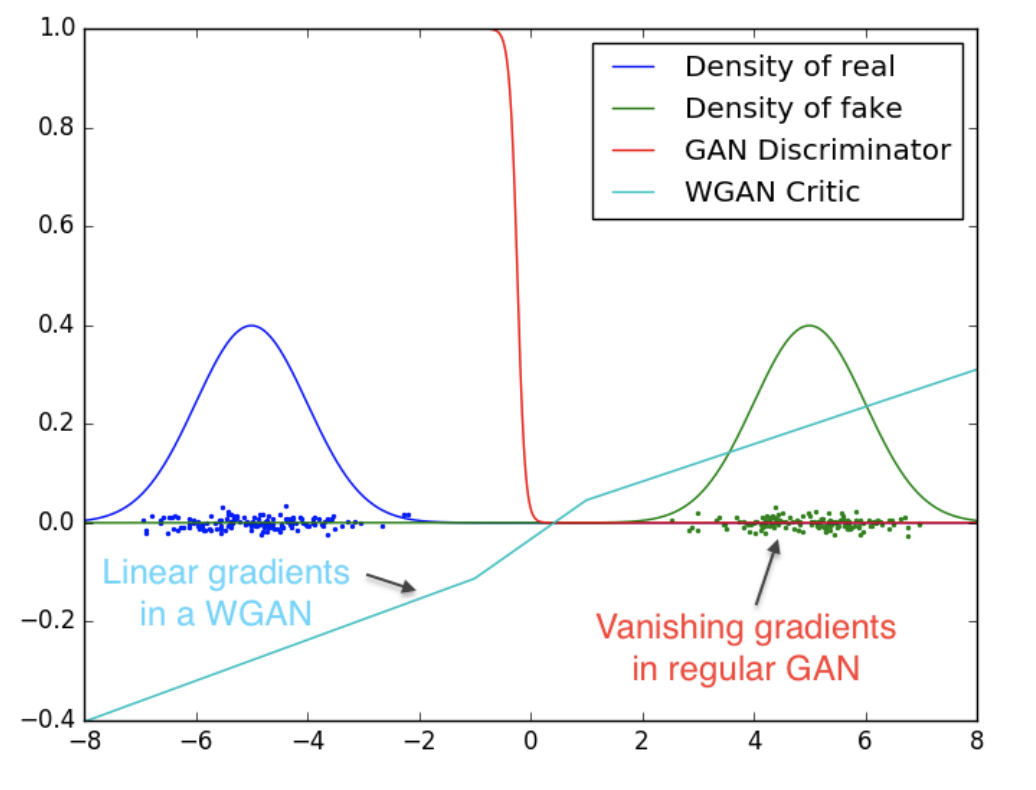
\includegraphics[width=0.65\textwidth]{resources/images/wgan1.png}
    \caption{The picture shows how WGAN performs compared to traditional GAN. WGAN can deliver strong gradients even if the two distributions do not overlap. The gradient signal vanishes for GANs.}
    \label{fig:wgan1}
\end{figure}

 
\subsubsection{Earthmover's Distance}

The Earthmover's Distance (EMD) \cite{emd} measures the work necessary to move the earth between two landmasses to make them equal. The following formula defines the EMD or Wasserstein-1 for two data distributions $ \mathbb{P}_{r} $  and $ \mathbb{P}_{g} $.\\

\begin{equation}
    W\left(\mathbb{P}_{r}, \mathbb{P}_{g}\right)=\inf _{\gamma \in \Pi\left(\mathbb{P}_{r}, \mathbb{P}_{g}\right)} \mathbb{E}_{(x, y) \sim \gamma}[\|x-y\|]
\end{equation}\\

The WGAN loss function approximates the EMD for the actual data distribution $ \mathbb{P}_{g} $ and a parameterized data distribution $ \mathbb{P}_{\theta} $. The condition is that the Discriminator $ f $ is Lipschitz-1.\\

\begin{equation}
    W\left(\mathbb{P}_{r}, \mathbb{P}_{\theta}\right)=\sup _{\|f\|_{L} \leq 1} \mathbb{E}_{x \sim \mathbb{P}_{r}}[f(x)]-\mathbb{E}_{x \sim \mathbb{P}_{\theta}}[f(x)]
\end{equation}\\

\subsubsection{Lipschitz Continuity}

The WGAN loss requires a Discriminator that is Lipschitz-1 constrained. The Lipschitz Continuity \cite{Eriksson2004lipschitz} describes the functions property how fast it can change.  A Lipschitz-continues function with a Lipschitz constant $ L_{f}=1 $ has the property that it continues at any point within a given interval $ I $. Further, it can only change by a maximum absolute value of 1 between two consecutive steps. That means that the absolute derivate at any point of the function is never higher than 1. Such a function is called Lipschitz-1.\\

\begin{equation}
    \left|f\left(x_{1}\right)-f\left(x_{2}\right)\right| \leq L_{f}\left|x_{1}-x_{2}\right| \quad \text { for all } x_{1}, x_{2} \in I
\end{equation}\\

A small Lipschitz constant $ L_{f} $ signifies that small changes in the function's input parameters yield small changes in its output. On the other hand, a high value for  $ L_{f} $ means that small changes in the input parameters can significantly affect the function's output.\\

In their work, they clip the Discriminator's weights by the factor $ c $ to enforce the Lipschitz constraint. They state that it is a terrible way to ensure the property and that the training's performance is sensitive to the choice of $ c $.

\subsubsection{Gradient Penalty}

For the reasons metioned above \citetitle{gulrajani2017wgangp} \cite{gulrajani2017wgangp} \citeauthor{gulrajani2017wgangp} demonstrate how an additional loss regularization term can replace the weight-clipping technique. They introduce a gradient penalty that does not suffer from the same weaknesses as weight-clipping.\\

\begin{equation}
    \lambda \underset{\hat{x} \sim \mathbb{P}_{\hat{x}}}{\mathbb{E}}\left[\left(\left\|\nabla_{\hat{\boldsymbol{x}}} f(\hat{\boldsymbol{x}})\right\|_{2}-1\right)^{2}\right]
\end{equation}\\

The equation above regularizes the Discriminator to have gradients with the norm of 1 almost everywhere. The gradient penalty randomly samples  $ x $ from $ \mathbb{P}_{\hat{x}} $ where $ \mathbb{P}_{\hat{x}} $ are the straight lines between $ \mathbb{P}_{g} $ and $ \mathbb{P}_{r} $.